\documentclass{article}
\usepackage{amsfonts, amsthm, amsmath, amssymb, mathtools, ulem, mathrsfs, physics, esint, siunitx, tikz-cd}
\usepackage{pdfpages, fullpage, color, microtype, cancel, textcomp, markdown, hyperref, graphicx}
\usepackage{enumitem}
\graphicspath{{./images/}}
\usepackage[english]{babel}
\usepackage[autostyle, english=american]{csquotes}
\MakeOuterQuote{"}
\usepackage{xparse}
\usepackage{tikz}
\usepackage{algpseudocode}

% fonts
\def\mbb#1{\mathbb{#1}}
\def\mfk#1{\mathfrak{#1}}
\def\mbf#1{\mathbf{#1}}
\def\tbf#1{\textbf{#1}}

% common bold letters
\def\bP{\mbb{P}}
\def\bC{\mbb{C}}
\def\bH{\mbb{H}}
\def\bI{\mbb{I}}
\def\bR{\mbb{R}}
\def\bQ{\mbb{Q}}
\def\bZ{\mbb{Z}}
\def\bN{\mbb{N}}

% brackets
\newcommand{\br}[1]{\left(#1\right)}
\newcommand{\sbr}[1]{\left[#1\right]}
\newcommand{\brc}[1]{\left\{#1\right\}}
\newcommand{\lbr}[1]{\left\langle#1\right\rangle}

% matrices
\newcommand{\m}[2][b]{\begin{#1matrix}#2\end{#1matrix}}
\newcommand{\arr}[3][\sbr]{#1{\begin{array}{#2}#3\end{array}}}

% misc
\NewDocumentCommand{\app}{O{x} O{\infty}}{\xrightarrow{#1\to#2}}
\renewcommand{\ss}{\subset}
\newcommand{\vn}{\varnothing}
\newcommand{\inv}{^{-1}}
\newcommand{\imp}{\implies}
\newcommand{\impleft}{\reflectbox{$\implies$}}
\renewcommand{\bar}{\overline}
\renewcommand{\d}{\partial}
\newcommand{\pf}{\tbf{Proof. }}

% greek
\newcommand{\e}{\epsilon}
\newcommand{\p}{\varphi}
\renewcommand{\t}{\theta}

% title
\title{Scientific Computing HW 12}
\author{Ryan Chen}
%\date{\today}
\setlength{\parindent}{0pt}


\begin{document}
	
\maketitle



\section*{Task 1}

Code: \url{https://github.com/RokettoJanpu/scientific-computing-1-redux/blob/main/hw12/task1.ipynb}

\begin{center}
	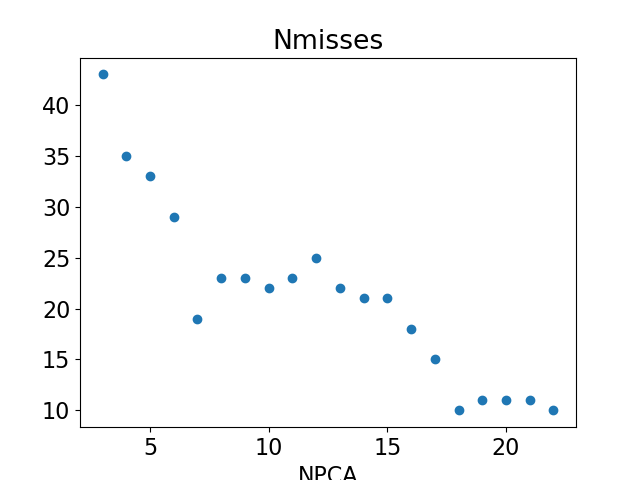
\includegraphics[scale=.5]{task1 misses}
\end{center}



\section*{Task 2}

Code: \url{https://github.com/RokettoJanpu/scientific-computing-1-redux/blob/main/hw12/task2.ipynb}

\begin{center}
	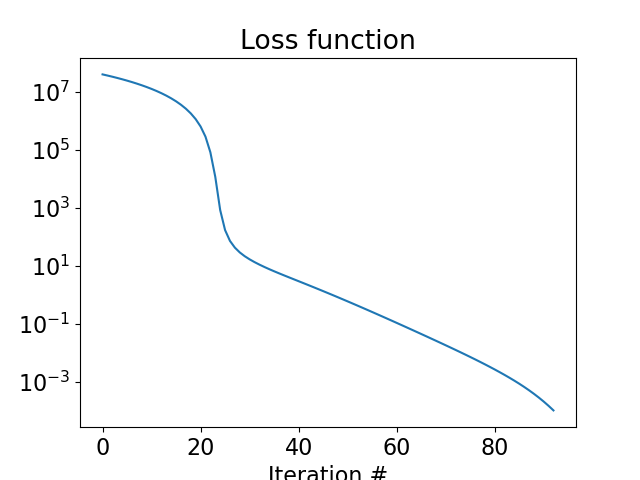
\includegraphics[scale=.5]{task2 loss}
	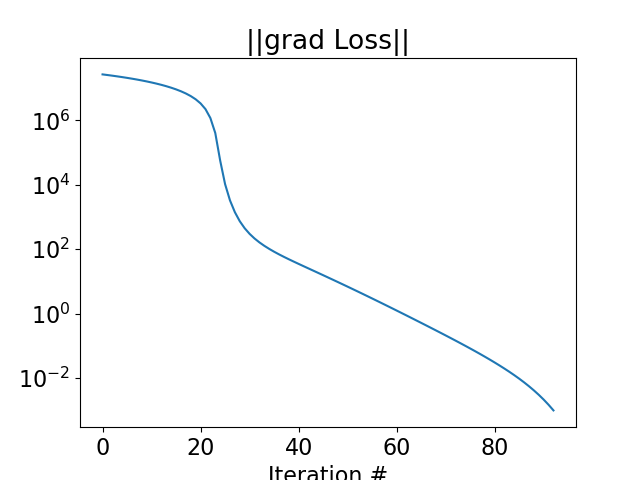
\includegraphics[scale=.5]{task2 gradnorm}
\end{center}



\section*{Task 3}

Code: \url{https://github.com/RokettoJanpu/scientific-computing-1-redux/blob/main/hw12/task2.ipynb}

	
\end{document}